%!TEX options=--shell-escape
\documentclass[tikz]{standalone}
\usepackage[T1]{fontenc}
\usepackage[utf8]{inputenc}
\usepackage{xcolor}
\usepackage{amsmath}
\usepackage{amssymb}
\usepackage{hyperref}
\usepackage{accsupp}    
\usepackage{graphicx}
\usepackage{mathtools}
\usepackage{pagecolor}
\usepackage{amsmath} % for \dfrac
\usepackage{tikz}
\tikzset{>=latex} % for LaTeX arrow head
\usepackage{braket}
\usepackage{pgfplots} 
\usepackage[edges]{forest}
\usetikzlibrary{patterns, backgrounds, arrows.meta}
\setlength{\parindent}{0cm}
\setlength{\parskip}{1em}

\usetikzlibrary{patterns}

\begin{document}
\def\rescale{0.142857}
\def\offset{0.035}

\begin{tikzpicture}[]

\path [use as bounding box] (-0.5- 2*\offset,-0.5 -2*\offset) rectangle (0.5 + 2*\offset,0.5 + 2*\offset);

\node[minimum height=3em,
      minimum width=3em,
           path picture={
               \node[yscale=-1,inner sep=0,outer sep=0] at (path picture bounding box.center){
                   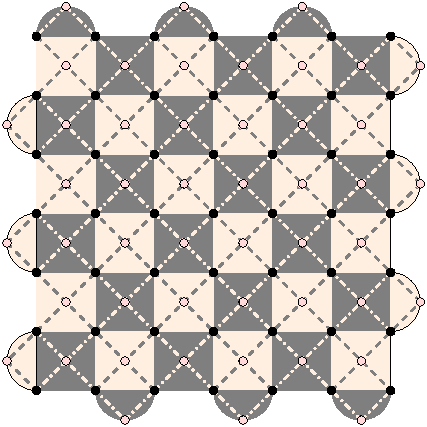
\includegraphics[scale=\rescale, angle=90, origin=c]{surface_code}
               };
           }] at (0, 0) {};

\end{tikzpicture} 
\end{document}

